%------------------------------------------------
% Quick reference. 
%------------------------------------------------
%
% Для вставки картинок:
%
%--------         Комманда
%
%\begin{figure}[H]
%	\includegraphics{img_name}
%	\caption{some caption}
%	\label{some_pic}
%\end{figure}
%
%--------        Переменные
%
% img_name     <- Название картинки в папке img.
% some_caption <- подпись картинки.
% label        <- лейбл нужен для ссылок на картинку.
% H            <- расположение картинки на странице.
% Чтобы сентрировать добавьте параметр \centering перед строчкой \includegraphics{}
% Чтобы вместить большой рисунок добавьте [width=\textwidth,height=\textheight,keepaspectratio] как параметр к \includegraphics{}
%--------         Пример
%
%\begin{figure}[H]
%   \centering
%	\includegraphics[width=\textwidth,height=\textheight,keepaspectratio]{pic1.jpg}
%	\caption{График зависимости какой-то хуйни}
%	\label{grapics1}
%\end{figure}
%
%------------------------------------------------
%
% Для референса по лейблу:
%
%--------         Комманда
%
% Для ссылки используется \eqref{ref}.
%
%--------        Переменные
%
% ref          <- указанный лейбл в директиве \label{ref}
%                 Ссылку можно сделать на любой объект имеющий \label{•}
%
%--------         Пример
%
% \eqref{graphics1}
%
%------------------------------------------------
%
% Для листинга кода:
%
%--------         Комманда
%
% \lstinputlisting[language=lang,mathescape=true]{src}
%--------        Переменные
%
% lang         <- язык на котором написан исходный код, например "python" или "C++".
% mathescape   <- если в исходниках есть формулы LaTeX, то они будут представлены как формулы.
% src          <- путь до файла исходников.
%
%--------         Пример
%
% \lstinputlisting[language=C++,mathescape=false]{./src/bullshit.cpp}
%
%------------------------------------------------
%
% Для вставки таблиц:
%
%--------
%\begin{table}[H]
%	\centering
%	\caption{ capt }
%	\begin{tabularx}{0.9\textwidth}{ | Y | Y | }
%		\hline
%		lines
%	\end{tabularx}
%	\label{tab1}
%\end{table}
%--------
% caption      <- Подпись таблицы.
% tab1         <- лейбл нужный для ссылки на таблицу.
% | Y | Y |    <- количество и формат столбцов.
% Y            <- Тип столбца.
%                 В данном случае определены кастомные столбцы Y (Спасибо Максиму Наумову)
% |            <- обозначает границы столбца.
%                 То есть, если будет указано |Y Y|, то столбцы внутри строк разделены не будут.
% H            <- То же самое, что и у картинок.
% lines        <- непосредственно элементы таблицы.
%                 Разделяются знаком "&", оканчивать каждую строку лучше \\ \hline
%
%--------         Пример
%\begin{table}[H]
%	\centering
%	\caption{ capt }
%	\begin{tabularx}{0.9\textwidth}{ | Y | Y | }
%		\hline
%		str1 & str2 \\ \hline
%		str1 & str2 \\ \hline
%		str1 & str2 \\ \hline
%		str1 & str2 \\ \hline
%		str1 & str2 \\ \hline
%	\end{tabularx}
%	\label{tab1}
%\end{table}
%------------------------------------------------

\documentclass[12pt, fleqn]{article}

\makeatletter
\renewcommand*\l@section{\@dottedtocline{1}{1.5em}{2.3em}}



%\includegraphics{universe}

\usepackage[utf8]{inputenc}
\usepackage[T2A]{fontenc}
\usepackage[russian]{babel} % указывает язык документа
\usepackage[left=3cm,right=2cm,top=2cm,bottom=2cm,bindingoffset=0cm]{geometry}
\usepackage{lastpage}
\usepackage{fancyhdr}
\usepackage{titlesec}
\usepackage{graphicx} % для вставки картинок
\usepackage[intlimits]{mathtools} % математические дополнения
\usepackage{amssymb}
\usepackage[tableposition=top]{caption}
\usepackage{subcaption}
\usepackage{indentfirst}
\usepackage{pythonhighlight}
\usepackage{listings}
\usepackage{tabularx}
\usepackage{tabulary}
\usepackage{multirow}
\usepackage{float}
\usepackage[figure,table]{totalcount}
\usepackage{diagbox}
\usepackage[german=guillemets]{csquotes}
\usepackage{fontspec} 
\usepackage{enumitem}
%\usepackege{xparse}
%\usepackage{mathptmx}% http://ctan.org/pkg/mathptmx
%\usepackage{showframe}
\usepackage{hyperref}

\setlength{\parindent}{1.2cm}

\setlength{\mathindent}{1.2cm}

\defaultfontfeatures{Ligatures={TeX},Renderer=Basic} 
\setmainfont[Ligatures={TeX,Historic}]{Times New Roman}

%\setlist[enumerate]{itemindent=\dimexpr\labelwidth+\labelsep\relax,leftmargin=0pt}

%\setlength{\section*}{0.5cm}
%\usepackage{minted}
%\usepackage{fancyvrb}
%\usepackage{newtxtext}

%\titleformat{\section}[hang]{\bfseries\LARGE\centering}{}{1em}{}

%\setlist[enumerate]{itemindent=\dimexpr\labelwidth+\labelsep\relax,leftmargin=0pt}
\setlist[enumerate,itemize]{leftmargin=0pt,itemindent=1.7cm}
\titleformat{\section}{\large\bfseries\centering}{\thesection}{0.5em}{\MakeUppercase}
\titleformat{\subsection}[block]{\bfseries\hspace{1em}}{\thesubsection}{0.5em}{}
%\setlength{\subsection*}{1.5cm}
%\setlength{\parindent}{4em}

%\setlength{\parindent}{1.5cm}

\captionsetup[figure]{labelfont={it},textfont={it},name={Рисунок},labelsep=endash, skip=5pt}
\captionsetup[table]{labelfont={it},textfont={it},name={Таблица},labelsep=endash,singlelinecheck=false, skip=5pt, margin=1cm}


%\renewcommand{\baselinestretch}{1.5}
\linespread{1.5} % полуторный интервал
\frenchspacing
\graphicspath{ {images/} }

  %-------------------------------------------
  % Переменные
  %-------------------------------------------

  \newcommand{\firstAuthorSurName}{Белоусов} 					                           % Фамилия автора.
  \newcommand{\firstAuthorInitials}{ А. А. } 					                           % Фамилия автора.
  \newcommand{\leftcolon}{Уравнения Математической Физики}
  \newcommand{\secondAuthorSurName}{Посоха} 					                           % Фамилия автора.
  \newcommand{\secondAuthorInitials}{ К. А.} 					                           % Фамилия автора.
  \newcommand{\teacherName}{Дегтярев А. А.}				                               % Имя преподавателя.
  \newcommand{\variantNumber}{40} 							                           % Номер варианта.
  \newcommand{\groupNumber}{6409-010302D} 				                               % Номер группы.
  \newcommand{\subjectTitle}{Отчет по курсовой работе}                                  % Название предмета.
  \newcommand{\taskTitle}{Дисциплина \enquote{Уравнения математической физики}} 		  % Название работы.
  \newcommand{\theme}{АНАЛИТИЧЕСКОЕ РЕШЕНИЕ КРАЕВЫХ ЗАДАЧ МАТЕМАТИЧЕСКОЙ ФИЗИКИ} 		  % Название работы.
  
  %-------------------------------------------
  % Ссылки в оглавлении
  %-------------------------------------------
  

\hypersetup{
    colorlinks,
    citecolor=black,
    filecolor=black,
    linkcolor=black,
    urlcolor=black
}

  %-------------------------------------------
  % Стиль футеров и хедеров
  %-------------------------------------------

\pagestyle{fancy}
\fancyhead[L, R]{}
\fancyfoot[L]{}
\fancyfoot[R]{}
\renewcommand{\footrulewidth}{0pt}
\renewcommand{\headrulewidth}{0pt}

%\renewcommand\subsectionfont{\normalfont\normalsize\bfseries}

\def\l@subsection{\@dottedtocline{2}{3.8em}{3.2em}}

% Для листинга

\lstset{
basicstyle=\footnotesize\ttfamily,
columns=fullflexible,
keywordstyle=\color{blue},
%frame=single,
breaklines=true,
numberstyle=\tiny\color{mygray},
postbreak=\mbox{\textcolor{red}{$\hookrightarrow$}\space},
showstringspaces=false,
}

\newcolumntype{Y}{>{\centering\arraybackslash}X}
\renewcommand{\tabularxcolumn}[1]{m{#1}} % Для вертикального центрировая табличных ячеек.

\begin{document}

%----------------------------------------------------------------------------------------
%	TITLE PAGE
%----------------------------------------------------------------------------------------
\pagenumbering{Alph}

\begin{titlepage}
							
	\center
							
	%------------------------------------------------
	%	Заголовки
	%------------------------------------------------
							
	\textsc{Министерство образования и науки Российской Федерации}\\[-0.15cm]
	\textsc{Федеральное государственное автономное образовательное учреждение \\[-0.15cm] высшего образования}\\[-0.15cm] 
	\textsc{«Самарский национальный исследовательский университет \\[-0.15cm] имени академика С.П.Королёва»}\\[0.25cm]
	\textsc{Факультет информатики}\\[0.1cm]
	\textsc{Кафедра технической кибернетики}\\[0.5cm]
						
	%------------------------------------------------
	%	Название работы
	%------------------------------------------------
							
	\vfill\vfill
						    
							
	{\large \textbf{\subjectTitle}}\\[0.3cm]
	
	{\large \taskTitle}\\[0.5cm]
						  
    {\large Тема: \enquote{\textbf{\theme}}}\\[0.5cm]

    \vfill
    
   {Вариант № \variantNumber}\\[0.5cm]


	\vfill\vfill
							
	\begin{minipage}{1\textwidth}
		\begin{center}
			\begin{tabularx}{\textwidth}{X l}
				Выполнил студент:        & \firstAuthorSurName \firstAuthorInitials \\
				Группа:                    & 6409                     		           \\
				Проверил:                  & \teacherName         		                \\
			\end{tabularx}
		\end{center}
	\end{minipage}
							
						
	%------------------------------------------------
	%	Дата
	%------------------------------------------------
							
	\vfill\vfill\vfill
					
	{\centering Самара \the\year}
							
							
\end{titlepage}

\pagenumbering{arabic}

\setcounter{page}{2}


%------------------------------------------------
%Задание
%------------------------------------------------

\section*{Задание к курсовой работе}
{
	\begin{enumerate}
	    \item Осуществить  математическую  постановку  краевой  задачи  для физического процесса, описанного в предложенном варианте курсовой работы.
        \item Используя  метод  разделения  переменных  (метод  Фурье),  получить решение краевой задачи в виде разложения в ряд Фурье по собственным функциям оператора Лапласа, соответствующим краевым условиям задачи.
        \item Провести анализ погрешности решения.
        \item Разработать  компьютерную  программу  расчета  функции-решения краевой  задачи  (суммирования  ряда  Фурье). При  расчете коэффициентов ряда использовать метод численного интегрирования, если  это  необходимо. Если необходимо, то разработать специальный программный модуль для вычисления используемых собственных чисел оператора Лапласа. Компьютерная  программа  должна  обеспечивать  возможность  диалогового режима  ввода  физических,  геометрических параметров  задачи,  числа суммируемых  элементов  ряда,  графическую  визуализацию  рассчитанного решения задачи.
        \item Оформить отчет о выполненной курсовой работе.
	\end{enumerate}
}
\newpage

\section*{\underline{\textit{Вариант} 40}}{
    Разработать программу расчета на промежутке времени $0<t \le T$ малых поперечных колебаний прямоугольной однородной мембраны шириной $l_x$ и длиной $l_y$. Колебания мембраны возбуждаются начальным отклонением
    $$u(x,y,t=0)=\alpha(x,y), 0 \le x \le l_x, 0 \le y \le l_y. $$ 
   
    Края мембраны $x=0, x=l_x, y=0$ и $y=l_y$ жестко закреплены, а реакция окружающей среды пренебрежимо мала. Начальные скорости точек мембраны равны нулю.
    
    Поверхностная плотность мембраны и величина натяжения, возникающего в ней в процессе колебаний, равны $\rho$ и $\eta$ соответственно.
   
    Для решения описанной задачи математической физики применить метод разделения переменных. Для расчетов использовать представление решения задачи в виде ряда Фурье по собственным функциям оператора Лапласа, удовлетворяющим соответствующим краевым условиям.
    
    При проведении расчетов использовать значения параметров $l_x, l_y, T, \rho, \eta,$ а также выражение функции $\alpha(x,y),$ указанные преподавателем.
    
    Значения параметров, указанные преподавателем:
    
    %{\renewcommand{\arraystretch}{1.6}%
    \bgroup
    \def\arraystretch{1.6}%  1 is the default, change whatever you need
    \begin{tabular}{rcl}
    $l_x$ & = & $4,$ \\ 
    $l_y$ & = & $1,$ \\
    $T$ & = & $10,$ \\
    $\rho$ & = & $1,$ \\
    $\eta$ & = & $1,$ \\
    $\alpha(x, y)$ & = & $ p(x,y)\sin(\dfrac{\pi y}{l_y}) $ \\
    $p(x,y)$ & = & $ \dfrac{x^2}{4} + x \quad $ \\

    \end{tabular} 
    \egroup

}

\newpage
\section*{РЕФЕРАТ}{
	\begin{center}
	\pageref{LastPage} страниц,
	\totalfigures\ рисунков,
	\totaltables\ таблиц,
	0 источников,
	1 приложение
	\end{center}
	
    \begin{center}
       УРАВНЕНИЯ МАТЕМАТИЧЕСКОЙ ФИЗИКИ, КРАЕВАЯ  ЗАДАЧА, УРАВНЕНИЕ ПОПЕРЕЧНЫХ КОЛЕБАНИЙ  ПРЯМОУГОЛЬНОЙ МЕМБРАНЫ,
        МЕТОД РАЗДЕЛЕНИЯ ПЕРЕМЕННЫХ, СОБСТВЕННЫЕ ФУНКЦИИ ОПЕРАТОРА ЛАПЛАСА, РЯД 
        ФУРЬЕ.     
    \end{center}
    

Целью курсовой работы является получение решения краевой задачи колебаний прямоугольной мембраны в виде разложения в ряд Фурье по собственным функциям оператора Лапласа и создание компьютерной программы для расчета функции-решения.

Для  получения  аналитического  решения  краевой  задачи  использован 
метод разделения переменных. Решение задачи получено в виде конечного ряда Фурье.

Разработана  компьютерная  программа,  обеспечивающая  расчет  и 
графическую  визуализацию  процесса колебаний мембраны.

Приведены  графические  результаты  численного  решения  задачи колебаний мембраны, а также анализ погрешности решения.

Программа  написана  на  языке Python в  среде  разработки PyCharm на операционной системе Windows. 

}

\newpage
\tableofcontents
\newpage
\phantomsection
\addcontentsline{toc}{section}{Введение}
%------------------------------------------------
%Введение
%------------------------------------------------

\section*{Введение}
{
Метод разделения переменных относится к классу аналитических
методов решения краевых задач математической физики. Характеризуя этот
метод необходимо выделить его достоинства и недостатки в сравнении с
другими методами.

К достоинствам метода разделения переменных следует отнести
возможность получения точного решения краевой задачи в виде ряда Фурье.
Такая форма решения задачи часто и весьма успешно используется для
теоретического исследования свойств этого решения. В случае достаточно
быстрой сходимости ряда Фурье она может с успехом использоваться для
численного моделирования физического процесса (явления).

К числу недостатков метода следует отнести его невысокую
универсальность. Этот метод весьма проблематично использовать для
решения нелинейных уравнений математической физики, уравнений с
переменными операторными коэффициентами, а также для решения краевых
задач в областях со сложными границами.

Суть метода разделения переменных состоит в факторизации по
каждой независимой переменной функции, определяющей решение
уравнения математической физики. Далее осуществляется переход к так
называемой задаче Штурма-Лиувилля, решение которой приводит к
получению собственных функций и соответствующих им собственных чисел
оператора Лапласа. Затем решение исходной задачи ищется в виде ряда
Фурье по этим собственным функциям.
    
В настоящей работе метод разделения переменных применен для
получения аналитической формы решения задачи описания процесса колебаний мембраны.
На основе этого результата разработан алгоритм и компьютерная программа
численного моделирования процесса колебаний мембраны.    
}
\newpage

%------------------------------------------------
% Начало основной части
%------------------------------------------------
\titleformat{\section}{\large\bfseries}{\thesection}{0.5em}{}
\titlespacing*{\section}{\parindent}{1ex}{1em}
\section{Постановка краевой задачи}
{

Построим математическую модель поперечных колебаний тонкой однородной мембраны.
Уравнение свободных поперечных колебаний мембраны имеет вид:
    \begin{equation}\label{source_func}
      \dfrac{\partial u}{\partial t} = \alpha^2(
      \dfrac{\partial u}{\partial x} + 
      \dfrac{\partial u}{\partial y}).
    \end{equation}

В условии задачи указано, что края мембраны жестко закреплены. Отсюда
    следуют граничные условия:
    \begin{equation}
    u|_{x=0}, \quad
    u|_{y=0},  \quad
    u|_{x=l_x}, \quad
    u|_{y=l_y} = 0.
    \end{equation}
    
По условию, в начальный момент времени отклонение мембраны задано функцией $\alpha(x, y)$, а начальная скорость точек мембраны равна нулю. Отсюда получаем начальные условия:
    \begin{align*}
        &  u|_{t=0} = p(x,y)\sin(\dfrac{\pi y}{l_y});\\        
        & \dfrac{\partial u}{\partial t}|_{t=0} = 0.
    \end{align*}
    
Производим следующую замену:
     \begin{equation}\label{change}
    	u(x,y,t) = \nu(x,t)\sin (\dfrac{\pi y}{l_y}).
    \end{equation}    
    
Подставляем в исходное уравнение, переходим к виду:
    \begin{equation}
         \dfrac{\partial \nu}{\partial t} = \alpha^2(\dfrac{\partial \nu}{\partial x}
        - \dfrac{\pi^2}{l_y}\nu(x, t)).
    \end{equation}
    
    Пересчитываем начальные условия для $\nu(x,y)$:
     \begin{align*}
        &  \nu|_{t=0} = p(x,y);\\        
        & \dfrac{\partial \nu}{\partial t}|_{t=0} = 0.
    \end{align*}
    
    
   Таким образом, имея уравнение, набор граничных и начальных условий, получим математическую модель, описывающую нашу задачу:
   		\begin{equation}
   		    u(x,y,t) = \nu(x,t)\sin (\dfrac{\pi y}{l_y});
   		\end{equation}
        \begin{equation}\label{eq15}
            \left\{
			\begin{split}
			& \dfrac{\partial \nu}{\partial t} = \alpha^2(\dfrac{\partial \nu}{\partial x}
        - \dfrac{\pi^2}{l_y}\nu(x, t)), \quad \le x \le \l_x; \\
			 &\nu|_{x=0}, \quad  
    \nu|_{x=l_x} = 0;\\
            &  \nu|_{t=0} = p(x,y);\\        
        	& \dfrac{\partial \nu}{\partial t}|_{t=0} = 0;
			\end{split}
			\right.
        \end{equation}
}
\newpage
\section{Аналитическое решение  краевой  задачи  и  получение  решения задачи в виде ряда Фурье}
{

Для решения поставленной задачи в уравнении \eqref{eq15} воспользуемся методом разделения переменных:
    \begin{equation}\label{eq16}
        \nu(x,t) = X(x)T(t).
    \end{equation}

Тогда уравнение \eqref{eq15} примет вид:    
    \begin{align*}
        &T''X = \alpha^2 \left(X''T - \dfrac{\pi^2}{l_y^2} XT \right);        
    \end{align*}
Разделим обе части на $a^2XT$ и получим следующее уравнение:
    \begin{equation}\label{eq17}
        \dfrac{T'}{\alpha^2T} = \dfrac{X''-\dfrac{\pi^2}{l_y^2}X}{X}.
    \end{equation}

В равенстве \eqref{eq17} можно заметить, что левая и правая части зависят только от $t$ и  $x$ соответственно. Тем самым, общая величина выражений - константа, которую мы возьмем равной $-\lambda^2$. Константа берется с отрицательным знаком, чтобы удовлетворять граничным условиям. Таким образом равенство \eqref{eq17} примет вид:

\begin{equation}\label{eq17}
        \dfrac{T'}{\alpha^2T} = \dfrac{
        X''-\dfrac{\pi^2}{l_y^2}X}{X} = -\lambda^2.
\end{equation}

Откуда получим два уравнения:
\begin{align*}
		& T''+\lambda^2\alpha^2T=0;\\
		& X''+(\lambda^2-\dfrac{\pi^2}{l_y^2})X = 0.
\end{align*}

Общие решения этих уравнений будут иметь следующий вид:
\begin{equation}\label{x_c}
	X(x) = A\cos(\sqrt{\dfrac{\pi^2}{l_y^2}-\lambda^2}x) + B\sin(\sqrt{\dfrac{\pi^2}{l_y^2}-\lambda^2}x),
\end{equation}
\begin{equation}\label{t_c}
	T(t) = C\cos(\alpha\lambda t) + D\sin(\lambda t),
\end{equation}
где $A, B, C, D$ - произвольные постоянные.

Подставляя полученные выражения $X(t), T(t)$ в равенство \eqref{eq16}, получаем:
\begin{equation}
	\nu(x,t) = (A\cos(\sqrt{\dfrac{\pi^2}{l_y^2}-\lambda^2}x) + B\sin(\sqrt{\dfrac{\pi^2}{l_y^2}-\lambda^2}x))(C\cos(\alpha\lambda t) + D\sin(\lambda t)).
\end{equation}

Произведем подбор постоянных $A, B$, так, чтобы полученное выражение удовлетворяло граничным условиям \eqref{eq15}. 

Для удовлетворяющей указанным условиям функции $X(x)$ должно выполняться $X(0)=0, X(l_x)=0$. Подставляя значения $x=0, x=l_x$ в \eqref{x_c}, получаем:
\begin{align*}
	& 0 = A\cos(0)+B\sin(0), &0 = A\cos(\sqrt{\dfrac{\pi^2}{l_y^2}-\lambda^2}l_x) + B\sin(\sqrt{\dfrac{\pi^2}{l_y^2}-\lambda^2}l_x).
\end{align*}

Из первого уравнения очевидно следует $A=0$. Из второго уравнения находим:
\begin{equation}\label{b_x}
	B\sin(\sqrt{\dfrac{\pi^2}{l_y^2}-\lambda^2}l_x) = 0.
\end{equation}
	$B\neq0$, так как в противном случае было бы $X=0$ и $u=0$, что противоречит условию. Следовательно, 
	\begin{align*}
	\sin(\sqrt{\dfrac{\pi^2}{l_y^2}-\lambda^2}l_x) = 0,
	\end{align*}
Откуда находим
	\begin{align*}
	&\sqrt{\dfrac{\pi^2}{l_y^2}-\lambda^2} = \dfrac{n\pi}{l_x}, n=1,2,..., \\
	&\lambda = \sqrt{\dfrac{n\pi^2}{l_x^2} + \dfrac{\pi^2}{l_y^2}}.
	\end{align*}
Итак, получаем подстановкой $\lambda$ в \eqref{b_x} вид функции $X(x)$:
	\begin{align*}
	X(x) = B\sin(\sqrt{\dfrac{n\pi^2}{l_x^2}}x) = B\sin(\dfrac{n\pi^2}{l_x^2}x).
	\end{align*}
Теперь, зная значение $\lambda$, можем записать для уравнения \eqref{t_c}:
	\begin{align*}
	&T(t) = C\cos(\alpha\sqrt{\dfrac{n\pi^2}{l_x^2} + \dfrac{\pi^2}{l_y^2}}t) + 
	D\sin(\alpha\sqrt{\dfrac{n\pi^2}{l_x^2} + \dfrac{\pi^2}{l_y^2}}t), n=1,2,..., \\
	\end{align*}
	
Подставляя для каждого $n$ полученные выражения в уравнение \eqref{eq16}, получаем решение исходного уравнения \eqref{eq15}, удовлетворяющее требуемым условиям. Обозначим это решение как $\nu_n(x,t)$:
	\begin{equation}
	\nu_n(x,t) = (C\cos(\alpha\sqrt{\dfrac{n\pi^2}{l_x^2} + \dfrac{\pi^2}{l_y^2}}t) + 
	D\sin(\alpha\sqrt{\dfrac{n\pi^2}{l_x^2} + \dfrac{\pi^2}{l_y^2}}t)) \sin(\dfrac{n\pi}{l_x}x)
	\end{equation}	 
	
Так как уравнение \eqref{eq15} является линейным и однородным, решение можно представить в виде ряда:
	\begin{equation}\label{series}
	\nu(x,t) = \sum_{n=1}^{\infty}{(C\cos(\alpha\sqrt{\dfrac{n\pi^2}{l_x^2} + \dfrac{\pi^2}{l_y^2}}t) + 
	D\sin(\alpha\sqrt{\dfrac{n\pi^2}{l_x^2} + \dfrac{\pi^2}{l_y^2}}t)) \sin(\dfrac{n\pi}{l_x}x)}.
	\end{equation}	 
	
Для удовлетворения начальным условиям требуется подобрать значения $C_n$ и $D_n$. По условию $\nu|_{t=0} = p(x,y)$. Соответственно, подставив в \eqref{series} значение $t=0$, получим:
	\begin{equation}\label{eq_p}
	p(x,y) = \sum_{n=1}^{\infty}{\sin(\dfrac{n\pi}{l_x}x)C_n}.
	\end{equation}
Если функция $p(x,y)$ такова, что в интервале $(0, l_x)$ ее можно разложить в ряд Фурье, условие \eqref{eq_p} будет выполняться при:
	\begin{equation}\label{cn_fin}
	C_n = \dfrac{2}{l_x}\int\limits_{0}^{l_x}{p(x)\sin(\dfrac{n\pi}{l_x}x)dx}.
	\end{equation}\
По условию $\dfrac{\partial \nu}{\partial t}|_{t=0} = 0$. Дифференцируем члены уравнения \eqref{series} по $t$ и учитываем это условие:
	\begin{equation}\label{dn_fin}
	0 = \sum_{n=1}^{\infty}{D_n\alpha\sqrt{\dfrac{n\pi^2}{l_x^2} + \dfrac{\pi^2}{l_y^2}}\sin(\dfrac{n\pi}{l_x}x)}.
	\end{equation}
Очевидно, что $\alpha\neq 0$, следовательно, из \eqref{dn_fin} получаем $D_n = 0$.  

Таким образом, приходим к аналитическому решению поставленной задачи \eqref{eq15} в следующем виде:
	\begin{align*}
  	&\dfrac{\partial u}{\partial t} = \nu(x,t)\sin (\dfrac{\pi y}{l_y}),
   	\end{align*}
   	\begin{equation}\label{final_series}
   	\nu(x,t) = \sum_{n=1}^{\infty}{(C_n\cos(\alpha\sqrt{\dfrac{n\pi^2}{l_x^2} + \dfrac{\pi^2}{l_y^2}}t)) \sin(\dfrac{n\pi}{l_x}x)},
	\end{equation}
	\begin{align*}
	C_n = \dfrac{2}{l_x}\int\limits_{0}^{l_x}{p(x)\sin(\dfrac{n\pi}{l_x}x)dx}.
	\end{align*}   	   		


%%========================================================================

\newpage
\section{Получение расчетной формулы}
{

Преподавателем была выдана функция $p(x,y)$, задающая начальное отклонение мембраны и значение поверхностной плотности $\rho$:
    \begin{align*}
        &p(x,y) = \dfrac{x^2}{4} + x, \quad \rho = 1. 
    \end{align*}
    
Размеры мембраны были заданы как $l_x=4, \quad l_y=1$.

Из вывода уравнения колебаний мембраны следует, что коэффициент $\alpha^2$ равен $\dfrac{1}{\rho}$. Следовательно, в нашем случае $\alpha=1$ и в дальнейших расчетах не оказывает влияния.

Вычислим значение коэффициента $C_n$ в сумме ряда \eqref{final_series} c учетом выданных значений.
	\begin{align*}
	&C_n = \dfrac{2}{l_x}\int\limits_{0}^{l_x}{p(x)\sin(\dfrac{n\pi}{l_x}x)dx} =  \dfrac{1}{2}\int\limits_{0}^{4}{p(x)\sin(\dfrac{n\pi}{4}x)dx} = 
	8\dfrac{n\pi\sin(n\pi) + 2\cos(n\pi) - 2}{n^3 \pi^3}.
	\end{align*}        
	
Перепишем решение задачи с учетом вычисленного коэффициента $C_n$ и выданных значений, получая итоговые расчетные формулы:
	\begin{align*}
  	&u(x,y,t) = \nu(x,t)\sin (\pi y),
   	\end{align*}
   	\begin{equation}\label{series_w_values}
   	\nu(x,t) = \sum_{n=1}^{\infty}{
   	8\dfrac{n\pi\sin(n\pi) + 2\cos(n\pi) - 2}{n^3 \pi^3}
   	\cos(\sqrt{\dfrac{n\pi^2}{16}+\pi^2}t)\sin(\dfrac{n\pi}{4}x)}.
	\end{equation}	 
} 

\newpage
\section{Оценка остатка ряда}
{
	Оценим остаток полученного ранее ряда Фурье \eqref{series_w_values}. Далее обозначаем $n$-ый элемент ряда как $D_n(x,t)$.
	Остаток оценивается как сумма элементов ряда, начиная с $N+1$-го:
	\begin{align*}
	|R_n| = \left|\beta\sum_{n=N+1}^{\infty}{D_n(x,t)}\right|.
	\end{align*}
	Тригонометрические функции не принимают значения по модулю больше единицы, поэтому могут быть заменены на 1:
	\begin{align*}
	&|\sin(n\pi)| < 1,\\
	&|\cos(n\pi)| < 1,\\
	&|\cos(\sqrt{\dfrac{n\pi^2}{16}+\pi^2}t)| < 1.
	\end{align*}
Тогда оценка остатка ряда приобретает следующий вид:
	\begin{equation}
	|R_n| \le \sum_{n=N+1}^{\infty}{\left|8\dfrac{n\pi+4}{n^3\pi^3}\right|} 
	\le 
	\dfrac{8}{\pi^2}\int\limits_{N}^{\infty}{\dfrac{dk}{k^2}} 
	+ \dfrac{32}{\pi^3}\int\limits_{N}^{\infty}{\dfrac{dk}{k^3}}
	\le 
	\left|8\dfrac{\pi N+16}{\pi^3 N^2 }\right| = \Phi(N).
	\end{equation}
	
Для контроля точности принимаем $\Phi(N) \le E$.

Отсюда получаем формулу для расчета числа суммирований ряда для достижения заданной точности:
\begin{equation}\label{precision}
	N = \dfrac{4(\sqrt{\pi E + 1}+1)}{\pi^2 E}.
\end{equation}
}

\newpage
\section{Экспериментальное исследование качества оценки остатка ряда }
{
Проведём экспериментальное исследование качества оценки остатка ряда следующим образом:
\begin{enumerate}
\item {
	Будем менять требуемую точность вычислений от $10^{-1}$ до $10^{-8}$.
}
\item {
	Для каждой требуемой точности рассчитаем $N_\text{избыточное}$ с помощью формулы \eqref{precision}.
}
\item {
	Рассчитаем $N_\text{достаточное}$, уменьшая количество слагаемых в сумме, начиная с $N_\text{избыточное}$ до тех пор, пока результат сохраняет требуемую точность.
}
\item {
	Шаги 1-3 проделаем для моментов времени $t = 0$, $t = 5$ и $t = 10000$. Это необходимо для того, чтобы проследить за изменением $N_\text{достаточное}$ на разных временных промежутках.
}
\end{enumerate}

\begin{table}[H]
\centering
\caption{Значения $N_\text{избыточное}$ и $N_\text{достаточное}$ при разных $\epsilon$ и $t$.}
\begin{tabularx}{\textwidth}{|Y|Y|Y|Y|Y|Y|Y|}
\hline
\multirow{2}{*}{$\epsilon$} & \multicolumn{2}{c|}{$t = 0$} & \multicolumn{2}{c|}{$t = 5$} & \multicolumn{2}{c|}{$t = 10000$} \\ \cline{2-7}
 & $N_\text{избыточное}$ & $N_\text{достаточное}$  & $N_\text{избыточное}$ & $N_\text{достаточное}$  & $N_\text{избыточное}$ & $N_\text{достаточное}$  \\ \hline
$10^{-1}$ & 2 & 0 & 2 & 0 & 2 & 0 \\ \hline
$10^{-2}$ & 8 & 0 & 8 & 0 & 8 & 2 \\ \hline
$10^{-3}$ & 25 & 0 & 25 & 2 & 25 & 3 \\ \hline
$10^{-4}$ & 78 & 0 & 78 & 9 & 78 & 5 \\ \hline
$10^{-5}$ & 246 & 0 & 246 & 25 & 246 & 8 \\ \hline
$10^{-6}$ & 778 & 0 & 778 & 65 & 778 & 15 \\ \hline
$10^{-7}$ & 2462 & 0 & 2462 & 152 & 2462 & 25 \\ \hline
$10^{-8}$ & 7784 & 0 & 7784 & 310 & 7784 & 38 \\ \hline
\end{tabularx}
\label{table_accuracy}
\end{table}

Как видно из таблицы \ref{table_accuracy} в моменты времени $t$ близкие к 0, достаточно небольшого количества слагаемых. Причиной этого является тот факт, что в начальный момент времени концентрация в трубке нулевая, а следовательно достаточно нуля слагаемых для описания системы.

Разница между моментами времени $t = 5$ и $t = 10000$ объясняется тем, что в итоговой формуле \eqref{u_solution} весь ряд умножается на $\mathrm{e}^{g_{2n + 1} t}$, где $g_{2n + 1}$ - отрицательная величина. Следовательно, в моменты времени $t \gg 0$ слагаемые убывают с большей скоростью, чем в моменты времени более близкие к моменту $t = 0$. Это означает что при больших $t$ достаточно меньшего количества слагаемых, так как каждый следующий член ряда убывает всё быстрее и быстрее.
}
\newpage

\newpage
\section{Результаты вычислительных экспериментов}
{

Ниже показан пример использования программы для моделирования теплового процесса в тонкой сфере.
Для расчета и визуализации функции $\omega(\theta,t)$ программа вызывается с аргументом ''pic''.

Для варьирования параметров, выданных преподавателем, следует передавать их как ''флаги'' программы.
Например, для изменения параметра ''a''($\alpha$) следует написать ''python umf.py pic --a=0.4'', теперь при расчетах
коэффициент теплопроводности $\alpha$ будет равен $0.4\left[\dfrac{\text{Вт}}{\text{см}^2 \cdot \text{K}}\right]$.
Стандартные параметры указаны преподавателем.

Для генерации видео программа должна быть запущена с параметром ''draw''.

Для расчетов коэффициентов $A_n$ программа запускается с аргументом ''find-a''.

Для вызова подсказок следует дописать ''-- --help'' в конец команды. Система подсказок работает для любой команды.
Все подсказки написаны на английском языке, для корректного встраивания текста программы в файл отчета.

Ниже, на рисунках \ref{grapics1}, \ref{grapics2}, \ref{grapics3} для начального условия $\psi_1(\theta)$ и \ref{grapics4}, \ref{grapics5}, \ref{grapics6} для $\psi_2(\theta)$, представлены выводы программы зависимости теплоты от угловой координаты в различные моменты времени $t$.


\begin{figure}[H]
    \centering                             
	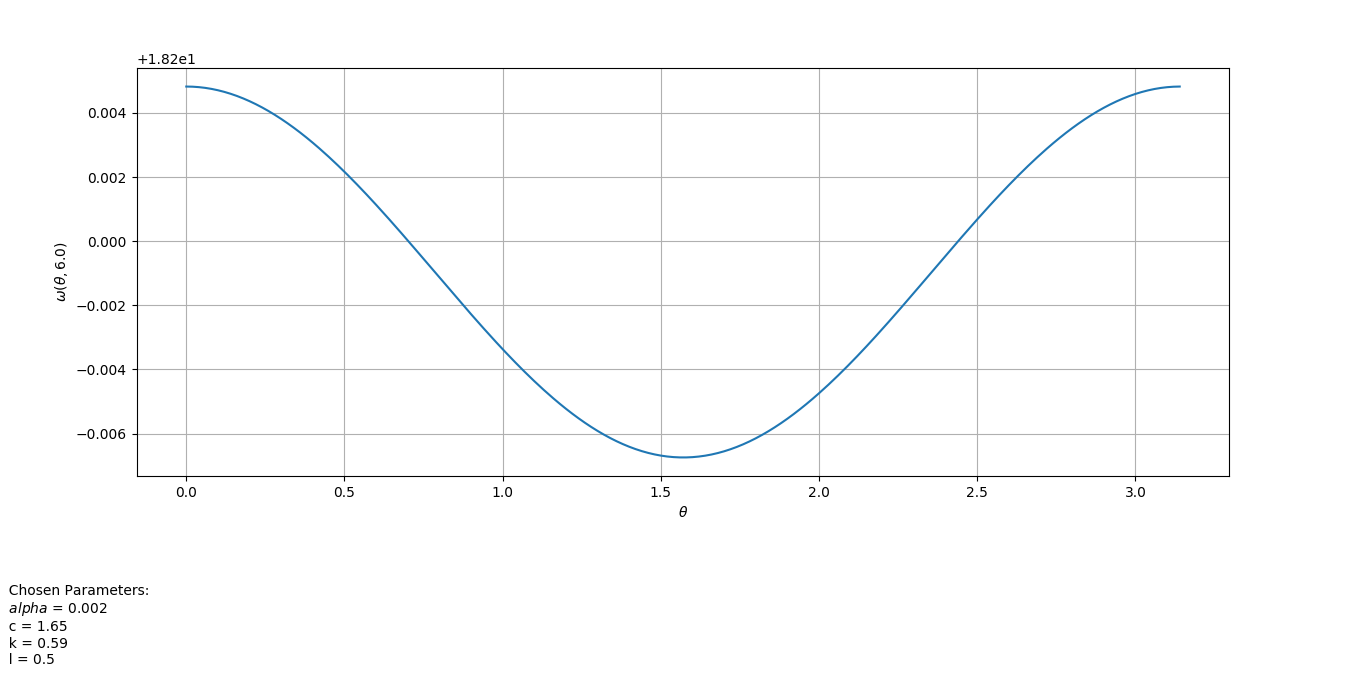
\includegraphics[width=\textwidth,height=\textheight,keepaspectratio]{kir/var_1_t_6.png}                 
	\centering\caption{ График температуры от времени t=6с при $\psi_1(\theta)$}
	\label{grapics1}                           
\end{figure}               

\begin{figure}[H]
    \centering                             
	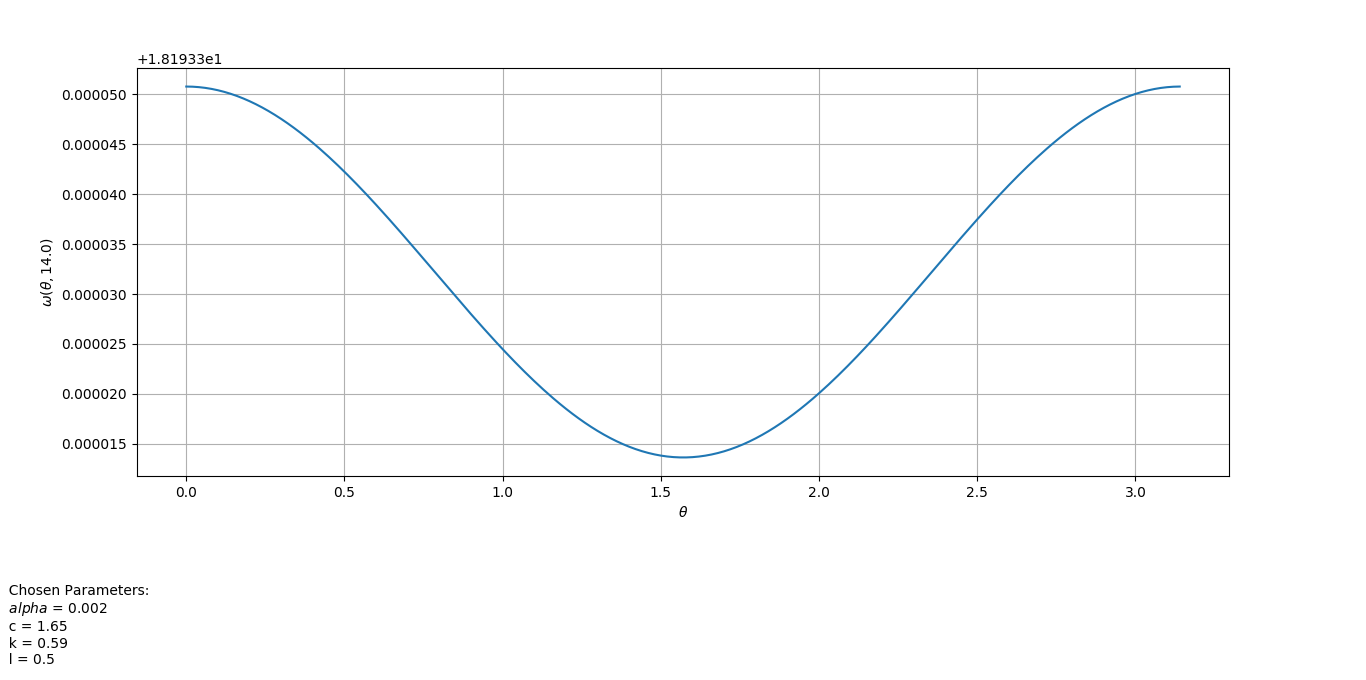
\includegraphics[width=\textwidth,height=\textheight,keepaspectratio]{kir/var_1_t_14.png}                 
	\caption{ График температуры от времени t=14с при $\psi_1(\theta)$}
	\label{grapics2}                           
\end{figure}                                  

\begin{figure}[H]
    \centering                             
	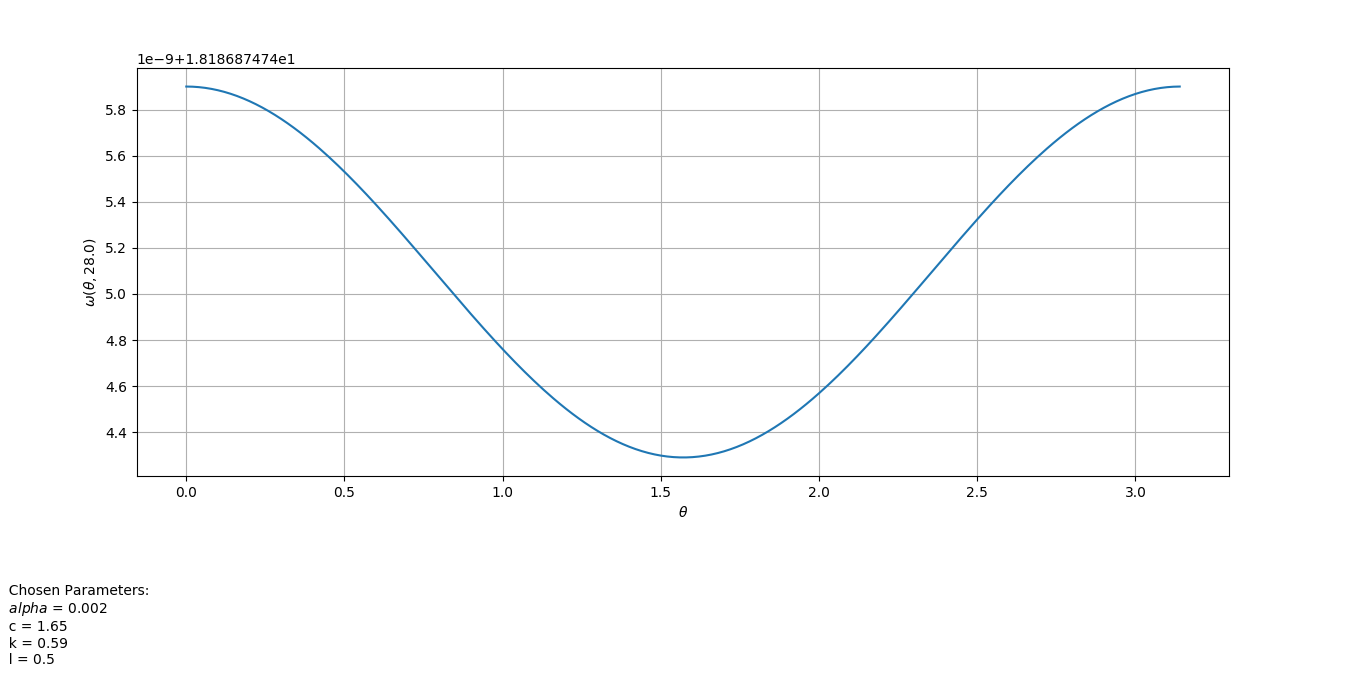
\includegraphics[width=\textwidth,height=\textheight,keepaspectratio]{kir/var_1_t_28.png}                 
	\caption{ График температуры от времени t=28с при $\psi_1(\theta)$}
	\label{grapics3}                           
\end{figure}              
\begin{figure}[H]
    \centering                             
	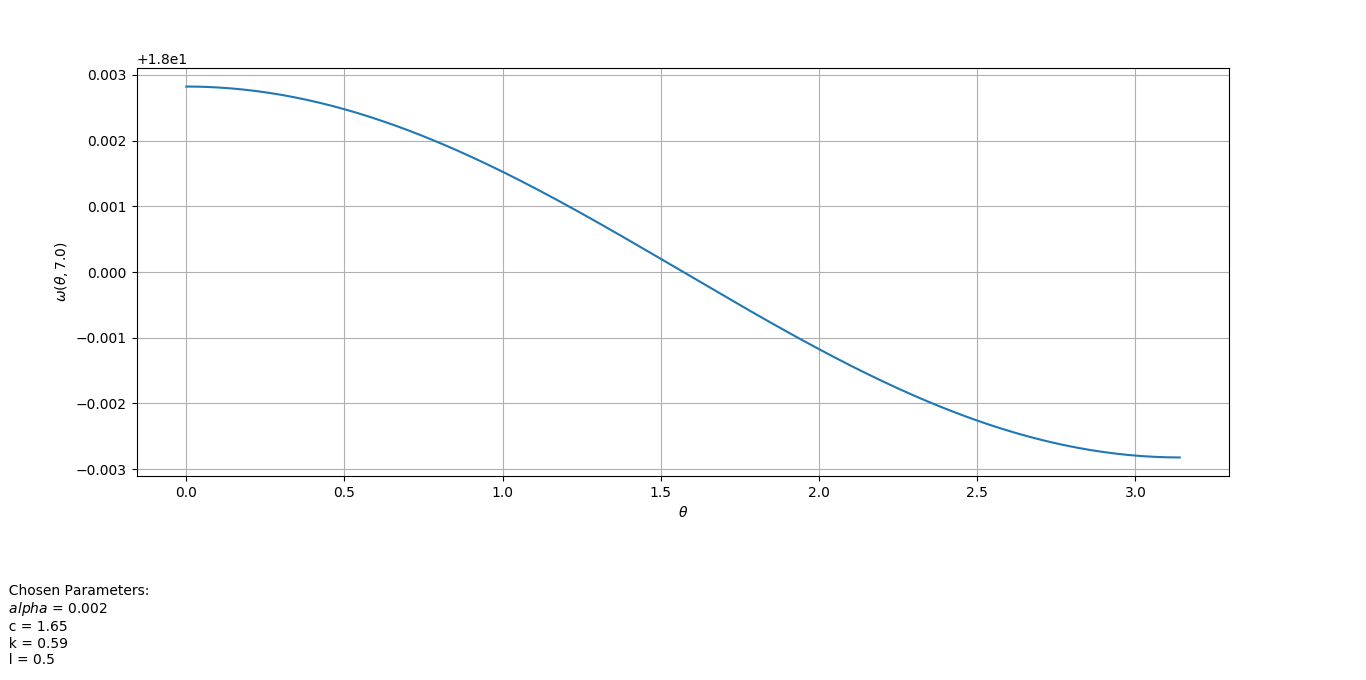
\includegraphics[width=\textwidth,height=\textheight,keepaspectratio]{pos/var_2_t_7.png}                 
	\caption{ График температуры от времени t=7с при $\psi_2(\theta)$}
	\label{grapics4}                           
\end{figure}               

\begin{figure}[H]
    \centering                             
	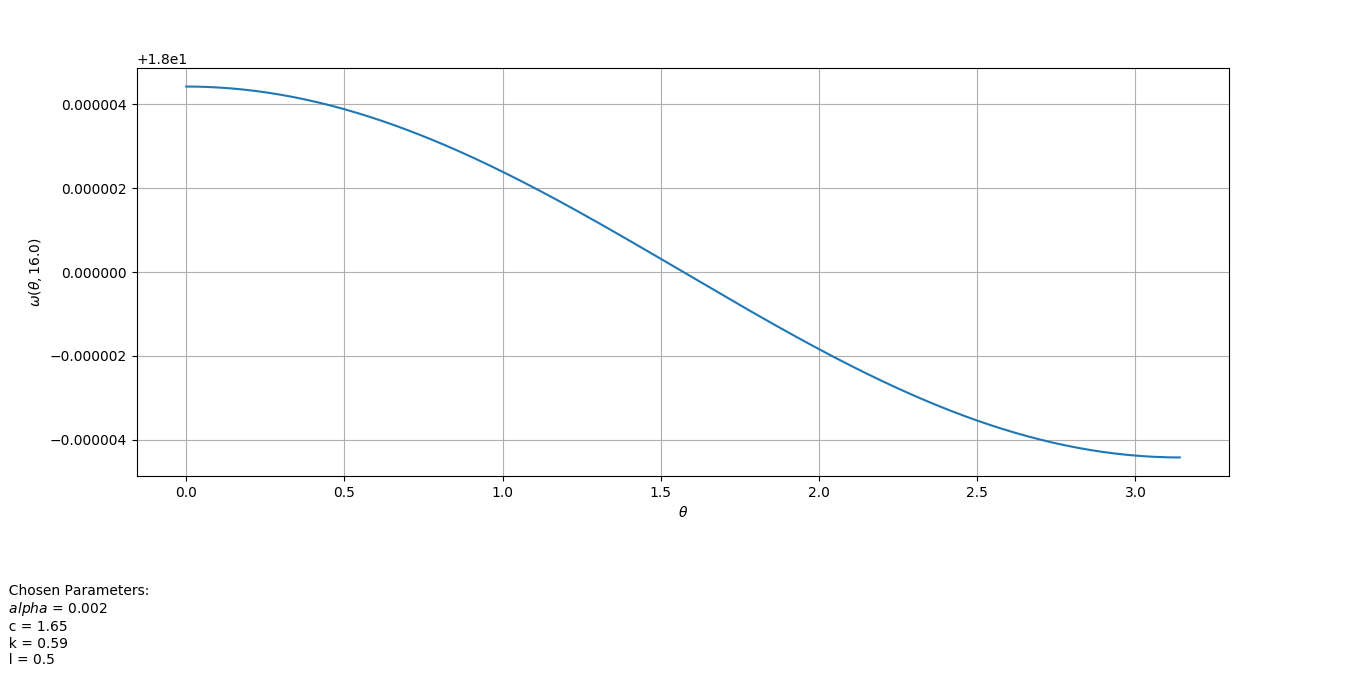
\includegraphics[width=\textwidth,height=\textheight,keepaspectratio]{pos/var_2_t_16.png}                 
	\caption{ График температуры от времени t=16с при $\psi_2(\theta)$}
	\label{grapics5}                           
\end{figure}                                  

\begin{figure}[H]
    \centering                             
	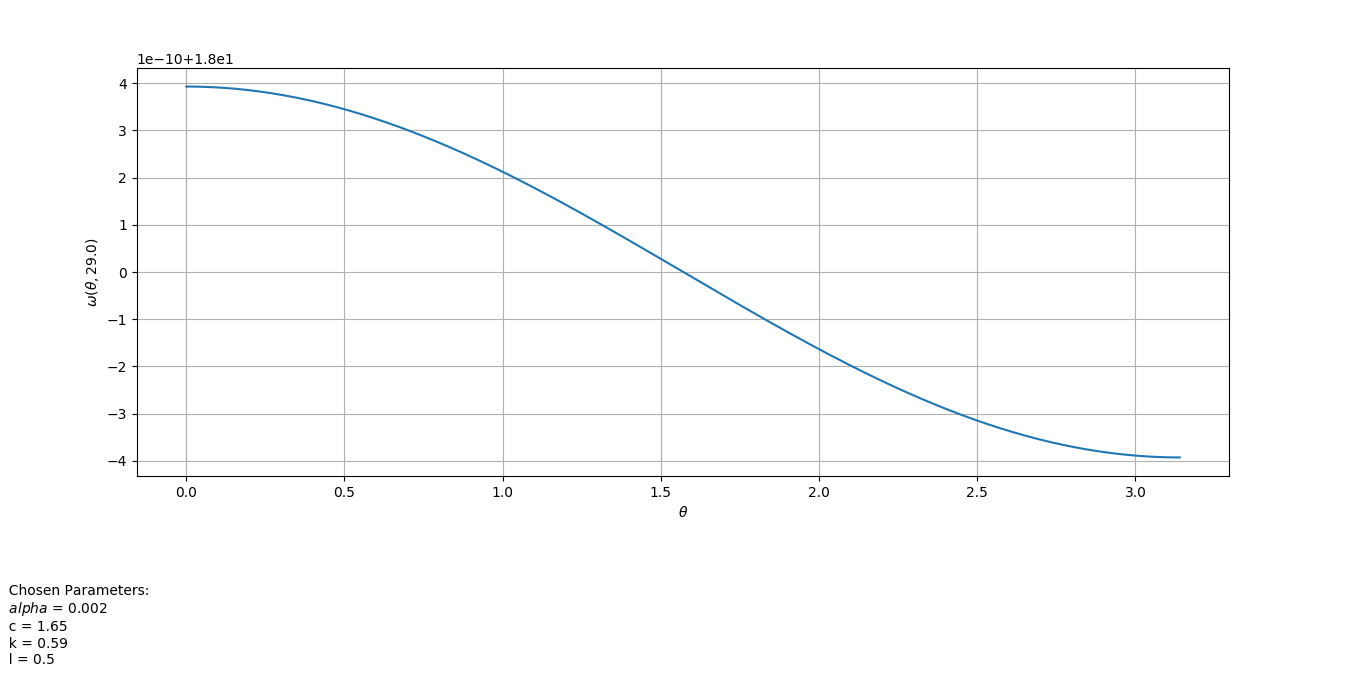
\includegraphics[width=\textwidth,height=\textheight,keepaspectratio]{pos/var_2_t_29.png}                 
	\caption{ График температуры от времени t=29с при $\psi_2(\theta)$}
	\label{grapics6}                           
\end{figure}              

На рисунках \ref{grapics7}, \ref{grapics8}, \ref{grapics9} для начального условия $\psi_1(\theta)$ и \ref{grapics10}, \ref{grapics11}, \ref{grapics12} для $\psi_2(\theta)$, представлены выводы программы зависимости теплоты от времени для различной угловой координаты $\theta$.  

\begin{figure}[H]
    \centering                             
	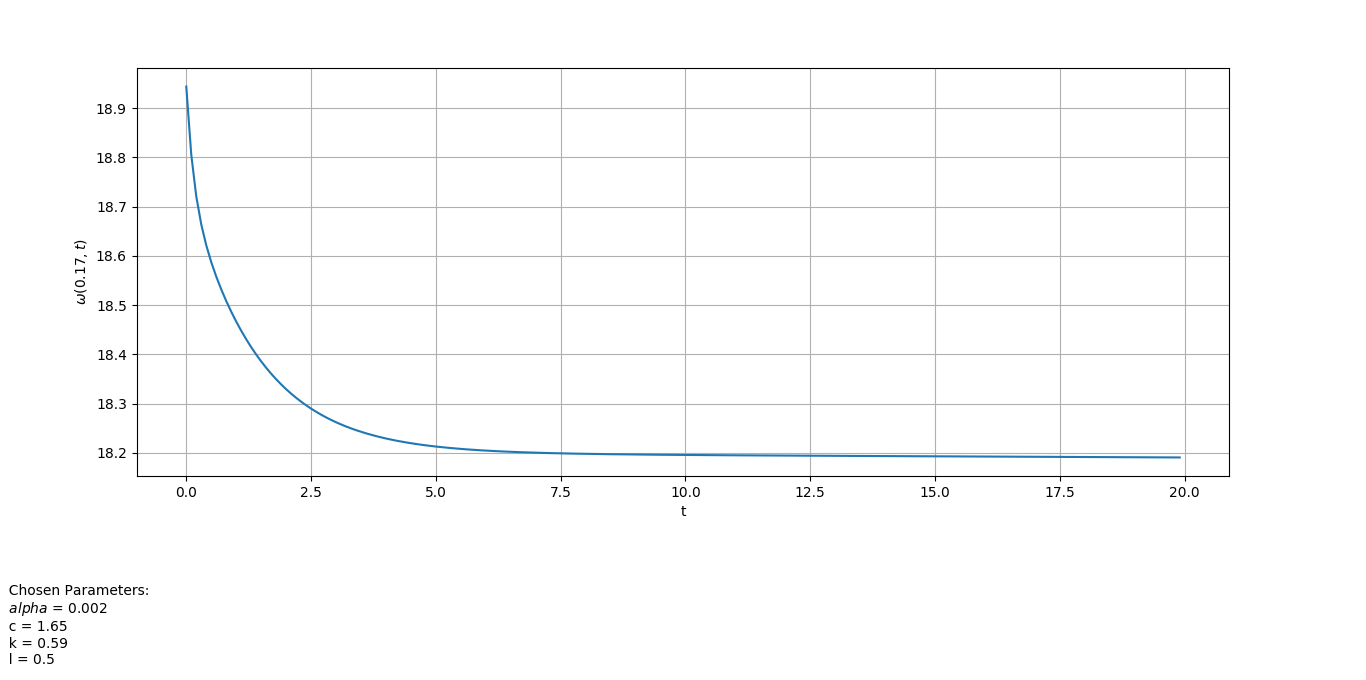
\includegraphics[width=\textwidth,height=\textheight,keepaspectratio]{kir/var_1_z_0t17.png}                 
	\centering\caption{ График температуры от времени $\theta=0.17$ при $\psi_1(\theta)$}
	\label{grapics7}                           
\end{figure}               

\begin{figure}[H]
    \centering                             
	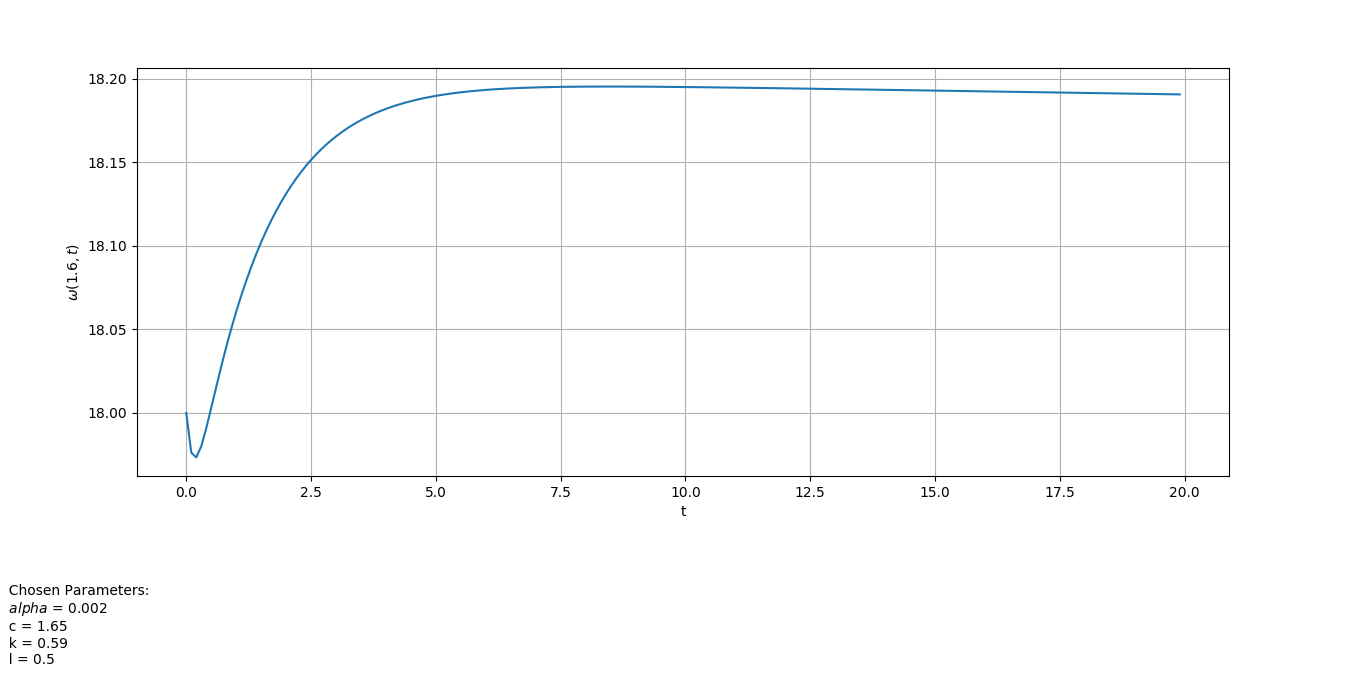
\includegraphics[width=\textwidth,height=\textheight,keepaspectratio]{kir/var_1_z_1t6.png}                 
	\caption{ График температуры от времени $\theta=1.6$ при $\psi_1(\theta)$}
	\label{grapics8}                           
\end{figure}                                  

\begin{figure}[H]
    \centering                             
	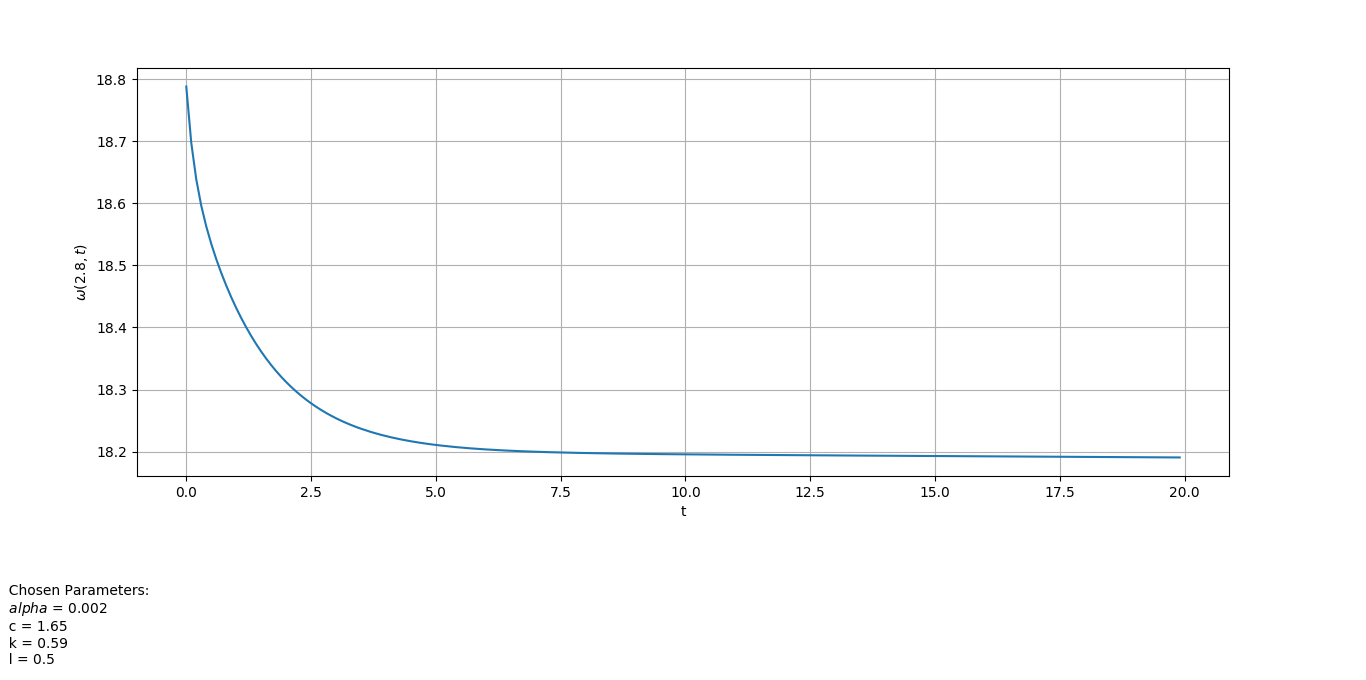
\includegraphics[width=\textwidth,height=\textheight,keepaspectratio]{kir/var_1_z_2t8.png}                 
	\caption{ График температуры от времени $\theta=2.8$ при $\psi_1(\theta)$}
	\label{grapics9}                           
\end{figure}              
\begin{figure}[H]
    \centering                             
	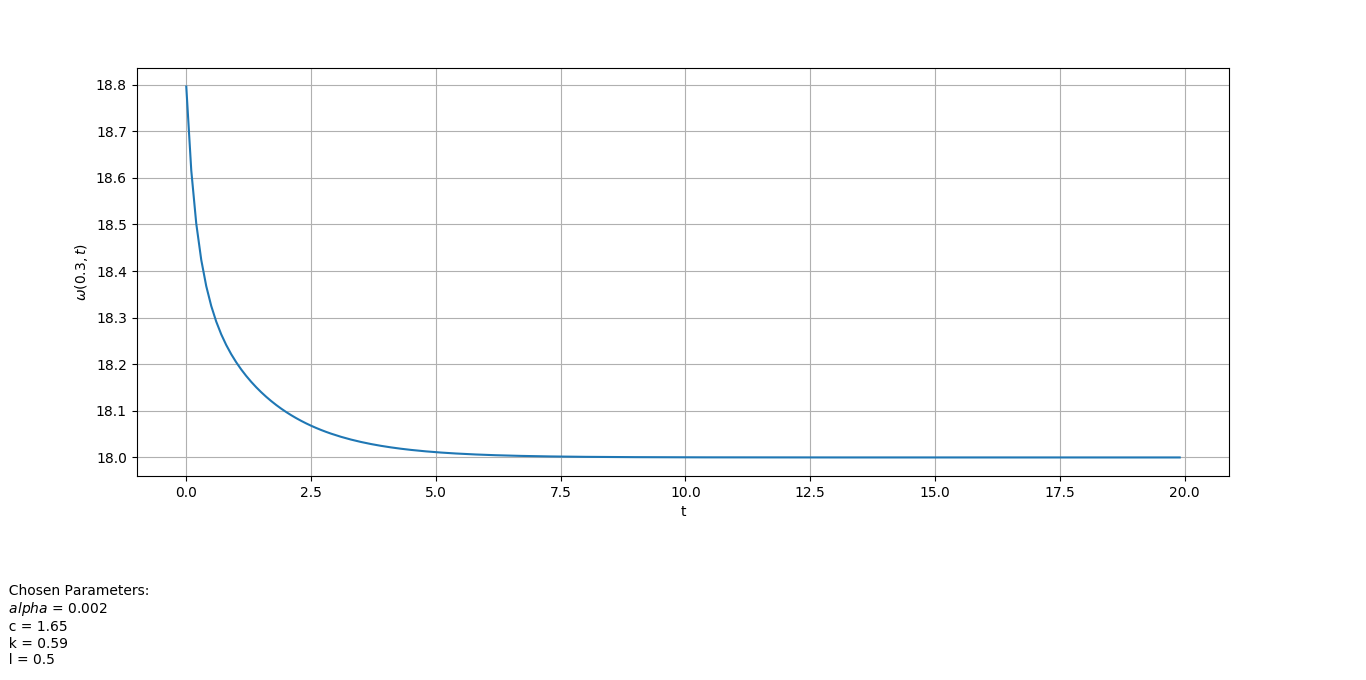
\includegraphics[width=\textwidth,height=\textheight,keepaspectratio]{pos/var_2_z_0t3.png}                 
	\caption{ График температуры от времени $\theta=0.3$ при $\psi_2(\theta)$}
	\label{grapics10}                           
\end{figure}               

\begin{figure}[H]
    \centering                             
	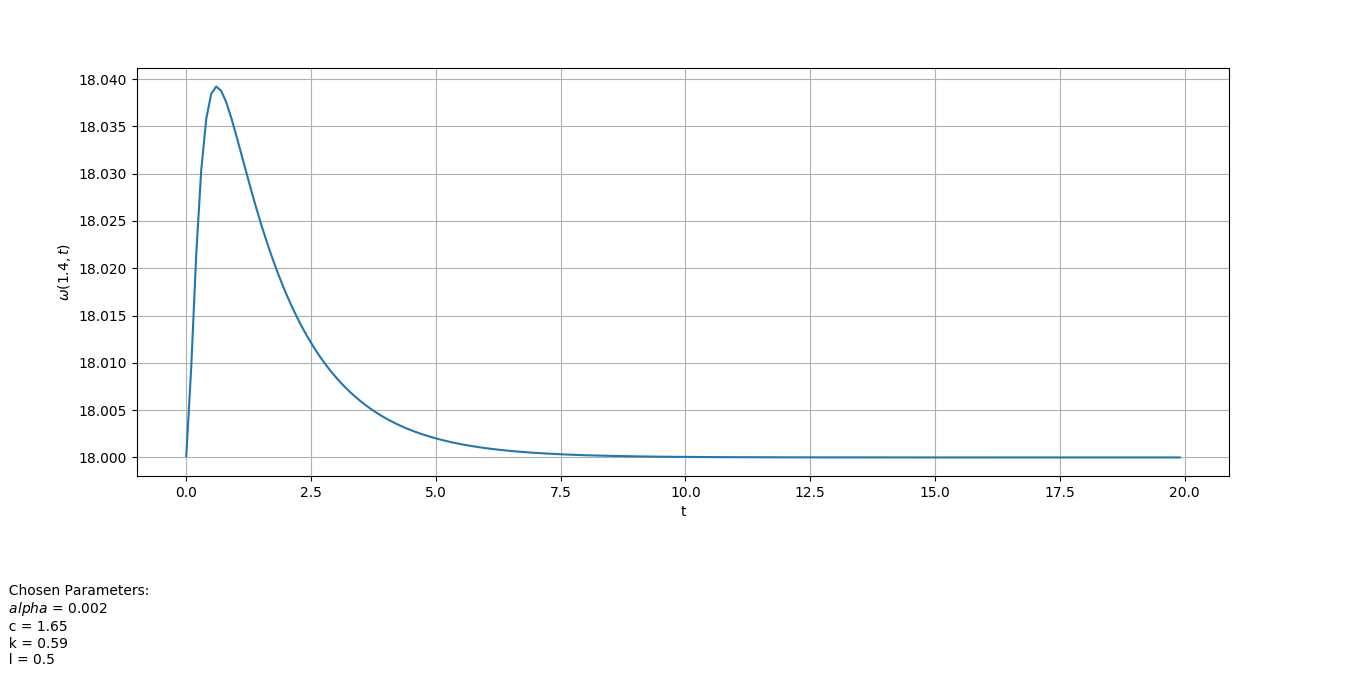
\includegraphics[width=\textwidth,height=\textheight,keepaspectratio]{pos/var_2_z_1t4.png}                 
	\caption{ График температуры от времени $\theta=1.4$ при $\psi_2(\theta)$}
	\label{grapics11}                           
\end{figure}                                  

\begin{figure}[H]
    \centering                             
	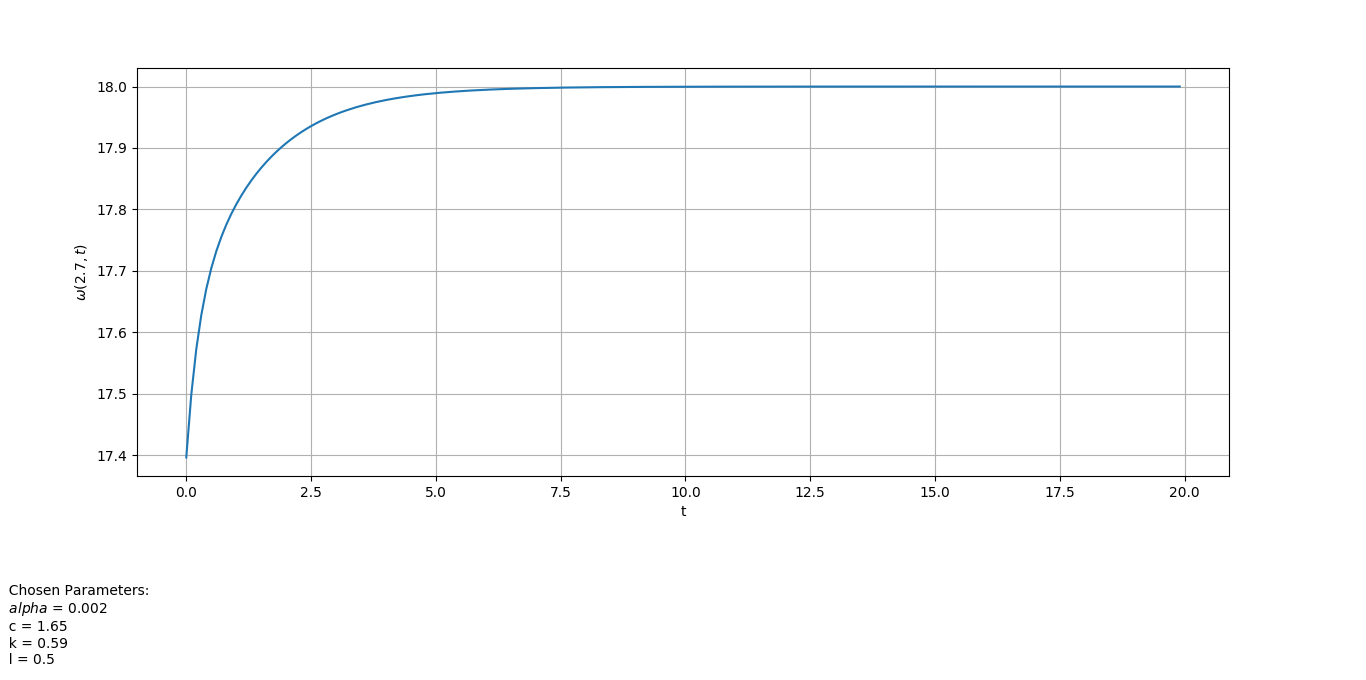
\includegraphics[width=\textwidth,height=\textheight,keepaspectratio]{pos/var_2_z_2t7.png}                 
	\caption{ График температуры от времени $\theta=2.7$ при $\psi_2(\theta)$}
	\label{grapics12}                           
\end{figure}              
                         
                     
    На рисунках с \ref{grapics7} по \ref{grapics12} можно заметить, что в любой точке сферы с увеличением времени
    будет устанавливаться тепловой баланс. А на рисунках с \ref{grapics1} по  \ref{grapics6} видна зависимость распределения температуры на оболочке сферы от начального условия. 
    
}


\newpage
\phantomsection
\addcontentsline{toc}{section}{Заключение}

%------------------------------------------------
% Заключение
%------------------------------------------------

\section*{Заключение}
{
    При выполнении данной работы были изучены аналитические методы решения краевой задачи теплопроводности. Составлена постановка краевой задачи, а также было получено аналитеческое решение в виде конечного ряда Фурье-Лежандра.
    
    
    В ходе работы для решения задачи была написана программа численного моделирования теплового процесса нагревания тонкой оболочки сферы. Данная программа выполняет расчеты темпиратуры с заданными параметрами и позволяет провести анализ погрешности решения для функции начального условия.
     
     
     Анализ полученных результатов показал, что была достигнута достаточно высокая точность решения, при относительно низкой вычислительной сложности.
     Что является хорошим результатом выполненной работы. 
    
}

\newpage
\phantomsection
\addcontentsline{toc}{section}{Список литературы}

%------------------------------------------------
% Список литературы
%------------------------------------------------

\section*{Список литературы}
{
	\begin{enumerate}
	\item \textbf{Дегтярев А.А.} Примеры построения и исследования разностных схем. – Электронное учебное пособие [Электронный ресурс]  / А.А Дегтярев, 2011. - 54с.\label{src1}
    \item \textbf{Тихонов А.Н., Самарский А.А}. Уравнения математической физики(5-е изд.) [Текст]
    / Тихонов А.Н., Самарский А.А. М.: Наука, 1977. - 742 с.\label{src2}
    	\item {Numpy and Scipy Documentation [Электронный ресурс]: Официальный сайт документации библиотек Numpy и Scipy. - URL: https://docs.scipy.org/doc/}\label{src3}
    	\item {MpMath Documentation [Электронный ресурс]: Официальный сайт документации библиотеки MpMath. - URL: http://mpmath.org/doc/current/}\label{src4}
	\end{enumerate}
}

%------------------------------------------------
% Приложения. Коды программ и.т.д.
%------------------------------------------------
\titleformat*{\section}{\large\bfseries\centering}

%\newpage
%\phantomsection
%\addcontentsline{toc}{section}{Приложение А Полиномы Лежандра}
%\section*{Приложение А}
%{	
%	\begin{center}
%	\textbf{Полиномы Лежандра}
%	\end{center}
%     
%    Полином Лежандра[\ref{src2}] — многочлен, который в наименьшей степени отклоняется от нуля в смысле среднего квадратического.
%    
%    Рекуррентная формула для вычисления $n$-го многочлена:
%    \begin{equation}
%    \left\{
%    \begin{split}
%    P_{0}(x)    &= 1; \\
%    P_{1}(x)    &= x; \\
%    P_{n+1}(x)  &= \dfrac{2n + 1}{n+1}xP_{n}(x) - \dfrac{n}{n+1}P_{n-1}(x). 
%    \end{split}
%    \right.
%    \end{equation}    
%    
%    Первые многочлены Лежандра:
%    \begin{align*}
%     &P_0(x) = 1; \\
%     &P_1(x) = x; \\
%     &P_2(x)=\frac{1}{2}(3x^2-1); \\
%     &P_3(x)=\frac{1}{2}(5x^3-3x); \\
%     &P_4(x)=\frac{1}{8}(35x^4-30x^2+3); \\
%     &P_5(x)=\frac{1}{8}(63x^5-70x^3+15x).
%    \end{align*}
%}
%
\newpage
\phantomsection
\addcontentsline{toc}{section}{Приложение Б Код программы}
\section*{Приложение Б}
{
	\begin{center}
	\textbf{Код программы}
	\end{center}
	\lstinputlisting[language=Python,mathescape=true]{./src/umf.py}
}
%
%\newpage
%\phantomsection
%\addcontentsline{toc}{section}{Приложение В Метод квадратур Гаусса-Лежандра}
%\section*{Приложение В}
%{
%\begin{center}
%	\textbf{Метод квадратур Гаусса-Лежандра}
%	\end{center}
%	
%	Метод квадратур Гаусса-Лежандра - метод численного интегрирования, в основе которого лежит метод квадратур Гаусса.
%	Особенностью метода является то, что он позволяет повысить алгебраический порядок точности, без увеличения числа 
%	используемых значений подынтегральной функции. 
%	Тем самым может быть достигнута максимальная точность для выбранного числа узлов интегрирования.
%	Численное интегрирование методом Гаусса вычисляется по формуле:
%	\begin{equation}
%	    I \approx \sum_{i=1}^{n}{\omega_i f(x_i)},
%	\end{equation}
%	где $x_i$ - узлы интегрирования, а $\omega_i$ - ненулевая константа, называемая ``вес квадратуры``.
%	
%	Для вычисления методом Гаусса-Лежандра веса вычисляются по следующей формуле:
%	\begin{equation}
%	    \omega_i = \dfrac{2}{(1-x^{2}_{i})\left[ P'_n(x_i) \right]^2},
%	\end{equation}
%	где $P'_n(x_i)$ - первая производная $n$-го полинома Лежандра, который описан в приложении А, 
%	$x_i$ - корни полинома Лежандра.
%	
%	Для нахождения производной многочлена Лежандра $n$-го порядка используется следующая рекуррентная формула:
%	\begin{equation}
%	    P'_n(x) = \dfrac{n}{x^2 - 1}\left(xP_{n}(x) - P_{n-1}(x) \right)
%	\end{equation}
%	
%    Многочлены Лежандра, в основном, не имеют аналитического решения и находятся через аппроксимирующие численные методы для нахождения корней.
%    На практике чаще всего используется метод касательной (Модификация метода Ньютона), который вычисляется по формуле:
%     \begin{equation}
%         x_{i+1} = x_i - \dfrac{P_n(x_i)}{P_n'(x_i)}
%     \end{equation}
%     Для начального приближения $i$-го корня полинома Лежандра степени $n$ берется
%     $$x_0 = \text{cos}\left(\pi\dfrac{i - \dfrac{1}{4}}{n + \dfrac{1}{2}}\right)$$
%     
%     Конечная формула для численного интегрирования:
%     \begin{equation}
%     \int\limits_{a}^{b}{f(x)} dx \approx \dfrac{b-a}{2}\sum_{i=1}^{n}{\omega_{i}f\left(\dfrac{b-a}{2}x_{i} + \dfrac{a+b}{2}\right)}
%     \end{equation}
%}
\end{document}
